\documentclass[12pt]{article}

\usepackage[a4paper,margin=2cm]{geometry}

\usepackage{amsmath}
\usepackage{amssymb}
\usepackage{mathtools}

\usepackage{listings}

\usepackage{booktabs} % For tables
\usepackage[table,xcdraw]{xcolor} % For tables

\usepackage{tikz} % TikZ
\usetikzlibrary{arrows.meta}

\usepackage{enumerate}
\usepackage{enumitem}

\usepackage{nameref}

\usepackage{xcolor}

\definecolor{codegreen}{rgb}{0,0.6,0}
\definecolor{codegray}{rgb}{0.5,0.5,0.5}
\definecolor{codepurple}{rgb}{0.58,0,0.82}
\definecolor{backcolour}{rgb}{0.95,0.95,0.92}

\lstdefinestyle{mystyle}{
    backgroundcolor=\color{backcolour},
    commentstyle=\color{codegreen},
    keywordstyle=\color{magenta},
    numberstyle=\tiny\color{codegray},
    stringstyle=\color{codepurple},
    basicstyle=\ttfamily\footnotesize,
    breakatwhitespace=false,
    breaklines=true,
    captionpos=b,
    keepspaces=true,
    numbers=left,
    numbersep=5pt,
    showspaces=false,
    showstringspaces=false,
    showtabs=false,
    tabsize=2
}

\lstset{style=mystyle}

\DeclarePairedDelimiter\abs{\lvert}{\rvert}
\DeclarePairedDelimiter\Abs{\lVert}{\rVert}

\usepackage{fancyhdr}

\pagestyle{fancy}
\lhead{\today}
\chead{Exercise 05\\Algorithmic Foundations of Data Science}
\rhead{Fabian Grob\\Simon Michau\\Til Mohr}

\setlength{\headheight}{50pt}

\begin{document}

\section*{Exercise 1}
\subsection*{(a)}
\begin{center}
\begin{tikzpicture}
		\node[draw, circle] (H) at (0,0) {H};
		\node[draw, circle] (B) at (-3,-3) {B};
		\node[draw, circle] (C) at (-3,3) {C};

		\path [->] (H) edge[loop right] node {$0.1$} (H);
		\path [->] (H) edge[bend right=20] node {$0.6$} (B);
		\path [->] (H) edge[bend right=20] node {$0.3$} (C);

		\path [->] (B) edge[bend right=20] node {$0.2$} (H);
		\path [->] (B) edge[loop below] node {$0.6$} (B);
		\path [->] (B) edge[bend right=20] node {$0.2$} (C);

		\path [->] (C) edge[bend right=20] node {$0.3$} (H);
		\path [->] (C) edge[bend right=20] node {$0.4$} (B);
		\path [->] (C) edge[loop above] node {$0.3$} (C);
\end{tikzpicture}
\end{center}
Transition matrix with row order (top to bottom) and column order (left to right) $H-B-C$:
\begin{equation*}
	Q \coloneqq \left[
		\begin{array}{ccc}
			0.1 & 0.6 & 0.3 \\
			0.2 & 0.6 & 0.2 \\
			0.3 & 0.4 & 0.3
		\end{array}
	\right]
\end{equation*}

\subsection*{(b)}
\begin{align*}
	\sum_{a \in {H,C,B}} q_{Ha} \cdot q_{aB} &= q_{HH} \cdot q_{HB} + q_{HB} \cdot q_{BB} + q_{HC} \cdot q_{CB} \\
	&= 0.1 \cdot 0.6 + 0.6 \cdot 0.6 + 0.3 \cdot 0.4 \\
	&= 0.06 + 0.36 + 0.12 \\
	&= 0.54
\end{align*}

\subsection*{(c)}
We have the following equations (also since $\pi$ is a left Eigenvector of $Q$ with Eigenvalue $1$):
\begin{equation}
	\pi_1 + \pi_2 + \pi_3 = 1
\end{equation}
\begin{equation}
	\pi \cdot Q = \pi
\end{equation}

Thus, we have the following equation system:
\begin{align*}
	\pi_1 + \pi_2 + \pi_3 &= 1 \\
	0.1 \cdot \pi_1 + 0.2 \cdot pi_2 + 0.3 \cdot \pi_3 &= \pi_1 \\
	0.6 \cdot \pi_1 + 0.6 \cdot pi_2 + 0.4 \cdot \pi_3 &= \pi_2 \\
	0.3 \cdot \pi_1 + 0.2 \cdot pi_2 + 0.3 \cdot \pi_3 &= \pi_3 \\
\end{align*}

Solving this, we get:
\begin{equation*}
	\pi \simeq \left(0.204082, 0.55101, 0.244897 \right)
\end{equation*}

\section*{Exercise 2}
\subsection*{(a)}
\subsection*{(b)}

\section*{Exercise 3}
\subsection*{(a)}
\subsection*{(b)}

\section*{Exercise 4}
\subsection*{(a)}
\subsection*{(b)}

\section*{Exercise 5}
\subsection*{(a)}
\subsection*{(b)}
\subsection*{(c)}


\section*{Appendix}\label{appendix}


\end{document}
